\documentclass[12pt,a4paper]{article}

\usepackage[T1]{fontenc}
\usepackage[utf8]{inputenc}
\usepackage[french]{babel}
\usepackage[margin=2.5cm]{geometry}
\usepackage{amsmath}
\usepackage{amssymb}
\usepackage{graphicx}
\graphicspath{{../../Images/}}
\usepackage{hyperref}

\usepackage{xcolor}
\usepackage{minted}

% --- Couleur Dracula ---
\definecolor{bg}{HTML}{282A36}

% --- Style minted ---
\usemintedstyle{dracula} % sinon mettre monokai si problème

\setminted{
    bgcolor=bg,
    fontsize=\small,
    linenos,
    breaklines,
    frame=none, % plus propre que frame=lines
    framesep=2mm
}

\title{Réunion du 01 avril 2026}
\author{Rodolphe Vivant}
\date{\today}

\begin{document}

\maketitle

\section{Sujets}
Liste des sujets abordés lors de la réunion :
\begin{itemize}
    \item Sujet 1 : Test sans anche
    \item Sujet 2 : Fonction $\gamma(t)$
    \item Sujet 3 : Calcul des résidus
    \item Sujet 4 : Résultats numériques comparées à OPENwind 
    \item Sujet 5 : Calcul du gradient
\end{itemize}

\section{Sujet 1 : Test sans anche}

\begin{minted}{python}
u0 = jnp.stack([
    jnp.stack([
        # ---- tilde p ----
        jnp.array([
            S_cells[i]/(c*S_star) * p0(xLs[i]),
            S_cells[i]/(c*S_star) * p0(xRs[i])
        ]),
        # ---- tilde v ----
        jnp.array([
            S_star/(c*S_cells[i]) * v0(xLs[i]),
            S_star/(c*S_cells[i]) * v0(xRs[i])
        ])
    ])
    for i in range(N)
], axis=0)
\end{minted}

\section{Sujet 2 : Fonction $\gamma(t)$}

voici les formules implémentées pour la fonction $\gamma(t)$ :
Il s'agit d'associer une montée en pression ($\text{attack(t)}$) et un plateau de pression ($\gamma_{\text{final}}$) pour modéliser l'entrée d'air dans l'instrument.
\begin{equation}
    \gamma(t) =
    \begin{cases}
        \text{attack}(t) & \text{pour } t < t_{\text{attack}}, \\
        \gamma_{\text{final}} & \text{pour } t \geq t_{\text{attack}}.
    \end{cases}
\end{equation}

Pour cela on implémente une fonction du type :

\begin{equation}
    \gamma(t) = (1-\omega_{\text{end}}(t))\text{attack}(t) + \omega_{\text{end}}(t)\gamma_{\text{final}}
\end{equation}

avec $\omega_{\text{end}}(t) = \sigma(\text{sharpness}(t-t_{\text{attack}}))$ et $\sigma(t)=\frac{1}{1+e^{-t}}$ la fonction sigmoïde. 

La fonction $\text{attack}(t)$ est calculer selon trois formes différentes : linéaire, exponentielle ou sigmoïde, selon les besoins de modélisation.

\begin{itemize}
    \item Cas linéaire : 
    \begin{equation}
        \text{attack}(t) = \gamma_{\text{final}} \text{clip}(\frac{t}{t_{\text{attack}}}, 0, 1)
    \end{equation}
    \item Cas exponentiel : 
    \begin{equation}
        \text{attack}(t) = \gamma_{\text{final}} (1 - e^{- t / \tau})
    \end{equation}
    avec $\tau = t_{\text{attack}} / \text{sharpness}$
    \item Cas sigmoïde : $\text{attack}(t) = \gamma_{\text{final}} \sigma(\text{sharpness} \cdot t)$
    \begin{equation}
        \text{attack}(t) = \frac{\gamma_{\text{final}}}{1+exp(-k(t-t_0))}
    \end{equation}
    avec $k=10/t_{\text{attack}}$ et $t_0= t_{\text{attack}}/2$
\end{itemize}



\begin{minted}{python}
import jax.numpy as jnp
import jax
from typing import Literal

@jax.jit(static_argnames=("shape",))
def pressure_at_mouth(
    gamma_final: float,
    t_attack: float = 0.2,
    sharpness: float = 10.0,
    t: jnp.ndarray = None,
    shape: Literal["exponential", "sigmoid", "linear"] = "exponential"
) -> jnp.ndarray:
    """
    Simule la pression d'air soufflée par un instrumentaliste.

    Paramètres
    ----------
    gamma_final : float
        Pression normalisée cible (plateau final).
    t_attack : float
        Durée de la montée en pression (secondes).
    sharpness : float
        Contrôle la transition vers le plateau (plus grand = plus rapide).
    t : jnp.ndarray
        Vecteur temps en secondes.
    shape : str
        Forme de l'attaque : "exponential", "sigmoid" ou "linear".

    Retourne
    --------
    gamma : jnp.ndarray  shape (N,)
        Pression normalisée au cours du temps.
    """
    assert shape in ["exponential", "sigmoid", "linear"]
    assert t is not None

    if shape == "exponential":
        tau    = t_attack / 100.0
        attack = gamma_final * (1.0 - jnp.exp(-t / tau))

    elif shape == "sigmoid":
        k      = 10.0 / t_attack
        t0     = t_attack / 2.0
        attack = gamma_final / (1.0 + jnp.exp(-k * (t - t0)))

    elif shape == "linear":
        attack = gamma_final * jnp.clip(t / t_attack, 0.0, 1.0)

    # Transition différentiable vers le plateau
    w_end     = jax.nn.sigmoid(sharpness * (t - t_attack))
    gamma     = (1.0 - w_end) * attack + w_end * gamma_final

    return t,gamma
\end{minted}

\newpage
\subsection{Résultats}

\begin{figure}[h!]
    \centering
    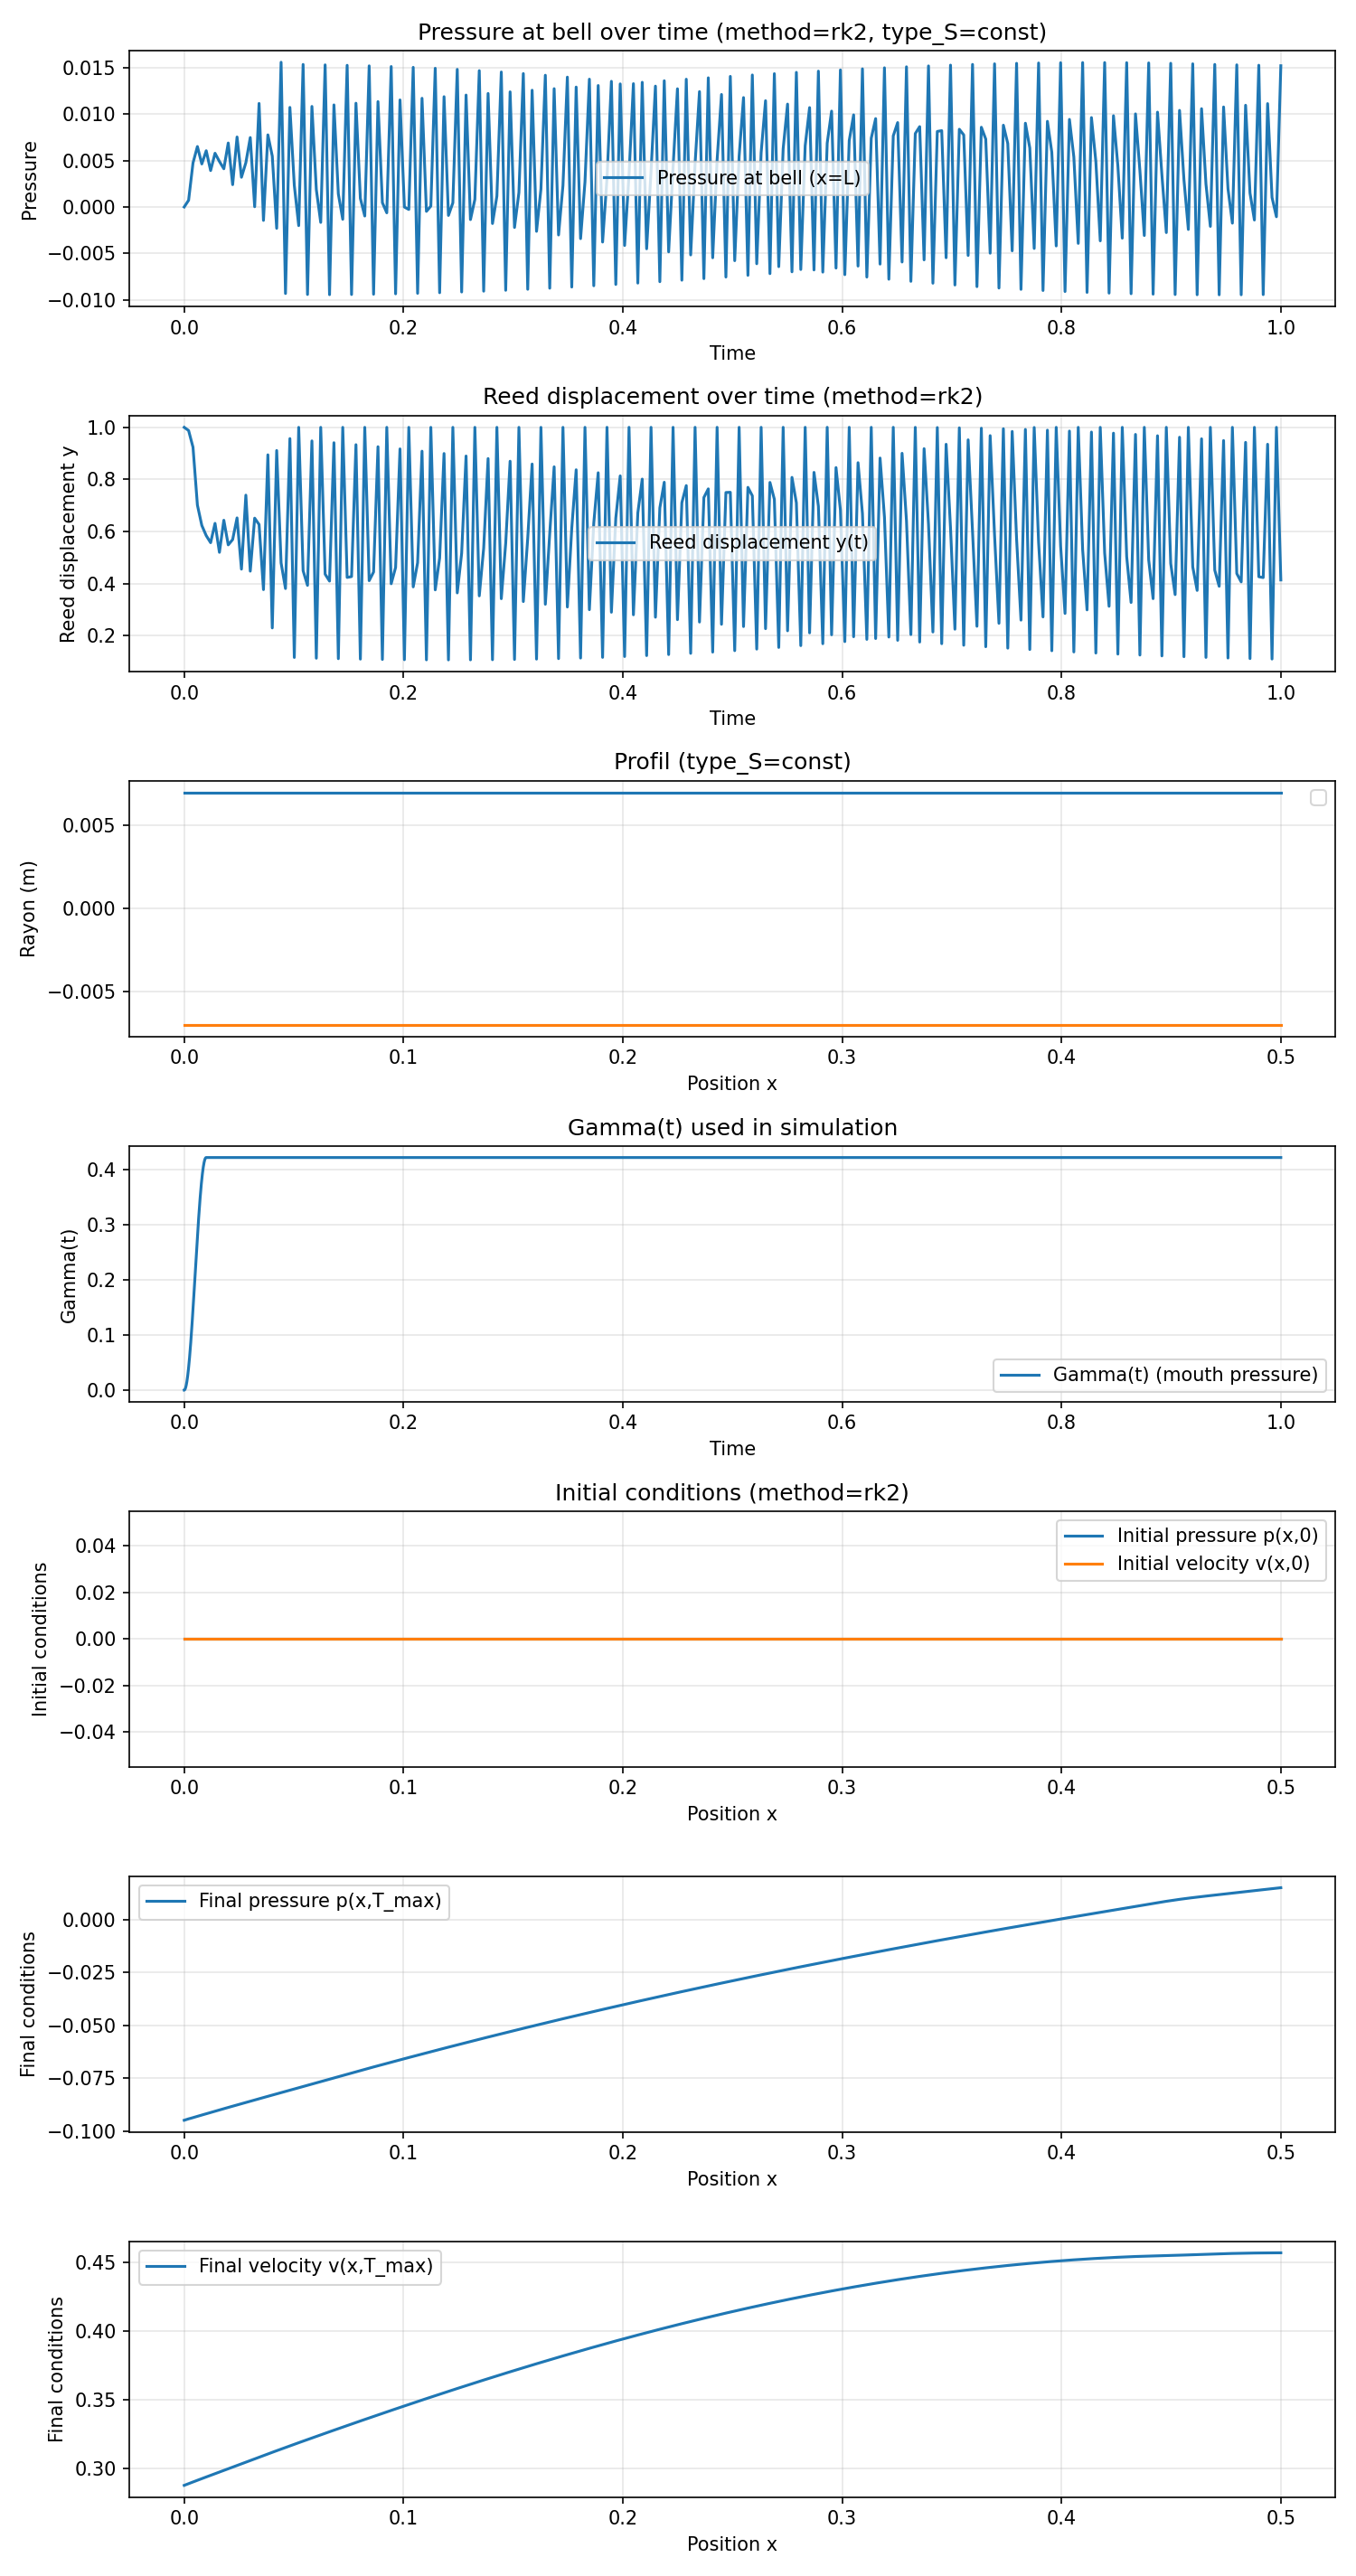
\includegraphics[width=0.7\textwidth]{pressure_and_reed_rk2_const.png}
    \caption{Résultats pour $\gamma(t)$ exponentiel dans le cas section constante.}
\end{figure}


\newpage
\section{Sujet 3 : Calcul des résidus}


\subsection{Développement mathématique}

\subsubsection{PDE}
\begin{equation}
    R_{PDE}(t,x) = \begin{bmatrix}
        \frac{\partial p_{tilde}}{\partial t} + \frac{\partial}{\partial x}\left(\frac{cS}{S^*} v_{tilde}\right) \\
        \frac{\partial v_{tilde}}{\partial t} + \frac{\partial}{\partial x}\left(\frac{cS^*}{S} p_{tilde}\right)
    \end{bmatrix}
\end{equation}

\subsubsection{pour ODE en $y$}
\begin{equation}
    R_{ODE}(t) = \frac{1}{\omega_r^2} \frac{d^2 y}{dt^2} + \frac{1}{Q_r \omega_r} \frac{dy}{dt} + y - 1 - \epsilon (\gamma(t) - p_L(t))
\end{equation}

\subsubsection{pour BC gauche}
\begin{equation}
    R_{BCL}(t) = -v_L(t) + \zeta l(y(t)) F(\gamma(t) - p_L(t)) + \epsilon \frac{\kappa}{\omega_r} \frac{dy}{dt}
\end{equation}

\subsubsection{pour BC droite}
\begin{equation}
    R_{BCR}(t) = -\frac{\beta}{Z} p_R(t) + v_R(t) + \sqrt{\alpha} \phi(t)
\end{equation}

\subsection{pour ODE en $\phi$}
\begin{equation}
    R_{\phi}=Z\partial_t \phi + \sqrt{\alpha} p_R
\end{equation}


\newpage
\subsection{Implémentation}

\begin{minted}{python}
    @jax.jit
    def compute_total_residual(
        u_snaps,      # (nsnaps, N, 2, 2)
        y_snaps,      # (nsnaps,)
        z_snaps,      # (nsnaps,)  d_t y stocké directement
        phi_snaps,    # (nsnaps,)
        gamma_snaps,  # (nsnaps,)
        S_cells,      # (N,)
        S_star,
        c,
        dt_snap,      # pas de temps entre snapshots
        h,            # taille d'une cellule
        beta, Z, alpha,
        eps, kappa,
        omega_r, Q_r,
        zeta,
        l
    ):
        """
        Calcule les résidus des équations (1a)-(1f) sur tous les snapshots.
        """

        # --------------------------------------------------
        # Variables centrales (on évite les bords temporels)
        # --------------------------------------------------
        u     = u_snaps[1:-1]     # (M, N, 2, 2)  M = nsnaps-2
        y     = y_snaps[1:-1]     # (M,)
        z     = z_snaps[1:-1]     # (M,)
        phi   = phi_snaps[1:-1]   # (M,)
        gamma = gamma_snaps[1:-1] # (M,)

        y_prev   = y_snaps[:-2]
        y_next   = y_snaps[2:]
        phi_prev = phi_snaps[:-2]
        phi_next = phi_snaps[2:]
        u_prev   = u_snaps[:-2]
        u_next   = u_snaps[2:]

        S_L = S_cells[0]
        S_R = S_cells[-1]

        # --------------------------------------------------
        # Conversions tilde vers physique aux bords
        # --------------------------------------------------
        pL = (c * S_star / S_L) * u[:, 0,  0, 0]   
        vL = (c * S_L   / S_star) * u[:, 0,  1, 0] 
        pR = (c * S_star / S_R) * u[:, -1, 0, 1]    
        vR = (c * S_R   / S_star) * u[:, -1, 1, 1]  

        # --------------------------------------------------
        # Dérivées temporelles
        # --------------------------------------------------
        # d_tt y par différences centrées sur snapshots
        y_tt  = (y_next - 2*y + y_prev) / dt_snap**2

        # d_t phi par différences centrées
        phi_t = (phi_next - phi_prev) / (2 * dt_snap)

        # d_t u par différences centrées (variables tilde)
        dt_u = (u_next - u_prev) / (2 * dt_snap)   # (M, N, 2, 2)

        # --------------------------------------------------
        # Résidu PDE - équations (1a)-(1b) en variables tilde
        # d_t p_tilde + d_x(cS/S* v_tilde) = 0
        # d_t v_tilde + d_x(cS*/S p_tilde) = 0
        # --------------------------------------------------
        # Flux aux interfaces intérieures (différences centrées en espace)
        # valeur droite de cellule j = u[:,j,:,1], valeur gauche de cellule j+1 = u[:,j+1,:,0]
        # interface j+1/2 : moyenne des deux

        # Valeur de p_tilde et v_tilde au centre de chaque cellule intérieure
        pt_center = 0.5 * (u[:, 1:-1, 0, 0] + u[:, 1:-1, 0, 1])  # (M, N-2)
        vt_center = 0.5 * (u[:, 1:-1, 1, 0] + u[:, 1:-1, 1, 1])  # (M, N-2)

        # Flux physiques : F_p = cS/S* * v_tilde 
        #                  F_v = cS*/S * p_tilde 
        flux_p = (c * S_cells[1:-1] / S_star) * vt_center    # (M, N-2)
        flux_v = (c * S_star / S_cells[1:-1]) * pt_center    # (M, N-2)

        # Dérivée spatiale par différences centrées (cellule j-1 à j+1)
        # on perd les cellules aux bords donc N-4 cellules intérieures
        dx_flux_p = (flux_p[:, 2:] - flux_p[:, :-2]) / (2 * h)   # (M, N-4)
        dx_flux_v = (flux_v[:, 2:] - flux_v[:, :-2]) / (2 * h)   # (M, N-4)

        # d_t p_tilde et d_t v_tilde au centre des cellules intérieures
        dt_pt = 0.5 * (dt_u[:, 1:-1, 0, 0] + dt_u[:, 1:-1, 0, 1])  # (M, N-2)
        dt_vt = 0.5 * (dt_u[:, 1:-1, 1, 0] + dt_u[:, 1:-1, 1, 1])  # (M, N-2)

        # Résidus PDE sur les cellules intérieures (N-4)
        res_pde_p = jnp.abs(dt_pt[:, 1:-1] + dx_flux_p)   # (M, N-4)
        res_pde_v = jnp.abs(dt_vt[:, 1:-1] + dx_flux_v)   # (M, N-4)

        # --------------------------------------------------
        # Résidu ODE anche - équation (1f)
        # 1/w² d_tt y + 1/(Qr w) d_t y + y - 1 = eps(gamma - p(0,t))
        # --------------------------------------------------
        res_ode = jnp.abs(
            y_tt / omega_r**2
            + z / (Q_r * omega_r)    # z = d_t y stocké directement 
            + y - 1.0
            - eps * (gamma - pL)
        )

        # --------------------------------------------------
        # Résidu BC gauche - équation (1e)
        # -v(0,t) + zeta l(y) F(gamma-p) + eps k/wr d_t y = 0
        # --------------------------------------------------
        res_bcL = jnp.abs(
            - vL
            + zeta * l(y) * F_func(gamma - pL)
            + eps * (kappa / omega_r) * z
        )

        # --------------------------------------------------
        # Résidu BC droite - équation (1d)
        # -beta/Z* p(L) + v(L) + sqert(alpha) phi = 0
        # --------------------------------------------------
        res_bcR = jnp.abs(
            - (beta / Z) * pR
            + vR
            + jnp.sqrt(alpha) * phi
        )

        # --------------------------------------------------
        # Résidu ODE phi - équation (1c)
        # Z* d_t phi + sqrt(alpha) p(L) = 0
        # --------------------------------------------------
        res_phi = jnp.abs(
            Z * phi_t + jnp.sqrt(alpha) * pR
        )

        return {
            "pde_p"   : res_pde_p,    # (M, N-4)
            "pde_v"   : res_pde_v,    # (M, N-4)
            "ode"     : res_ode,      # (M,)
            "bc_left" : res_bcL,      # (M,)
            "bc_right": res_bcR,      # (M,)
            "phi"     : res_phi,      # (M,)
        }
\end{minted}


\newpage
\subsection{Résultats}

\subsubsection{Cas $S(x$ constant)}

\begin{figure}[h]
    \centering
    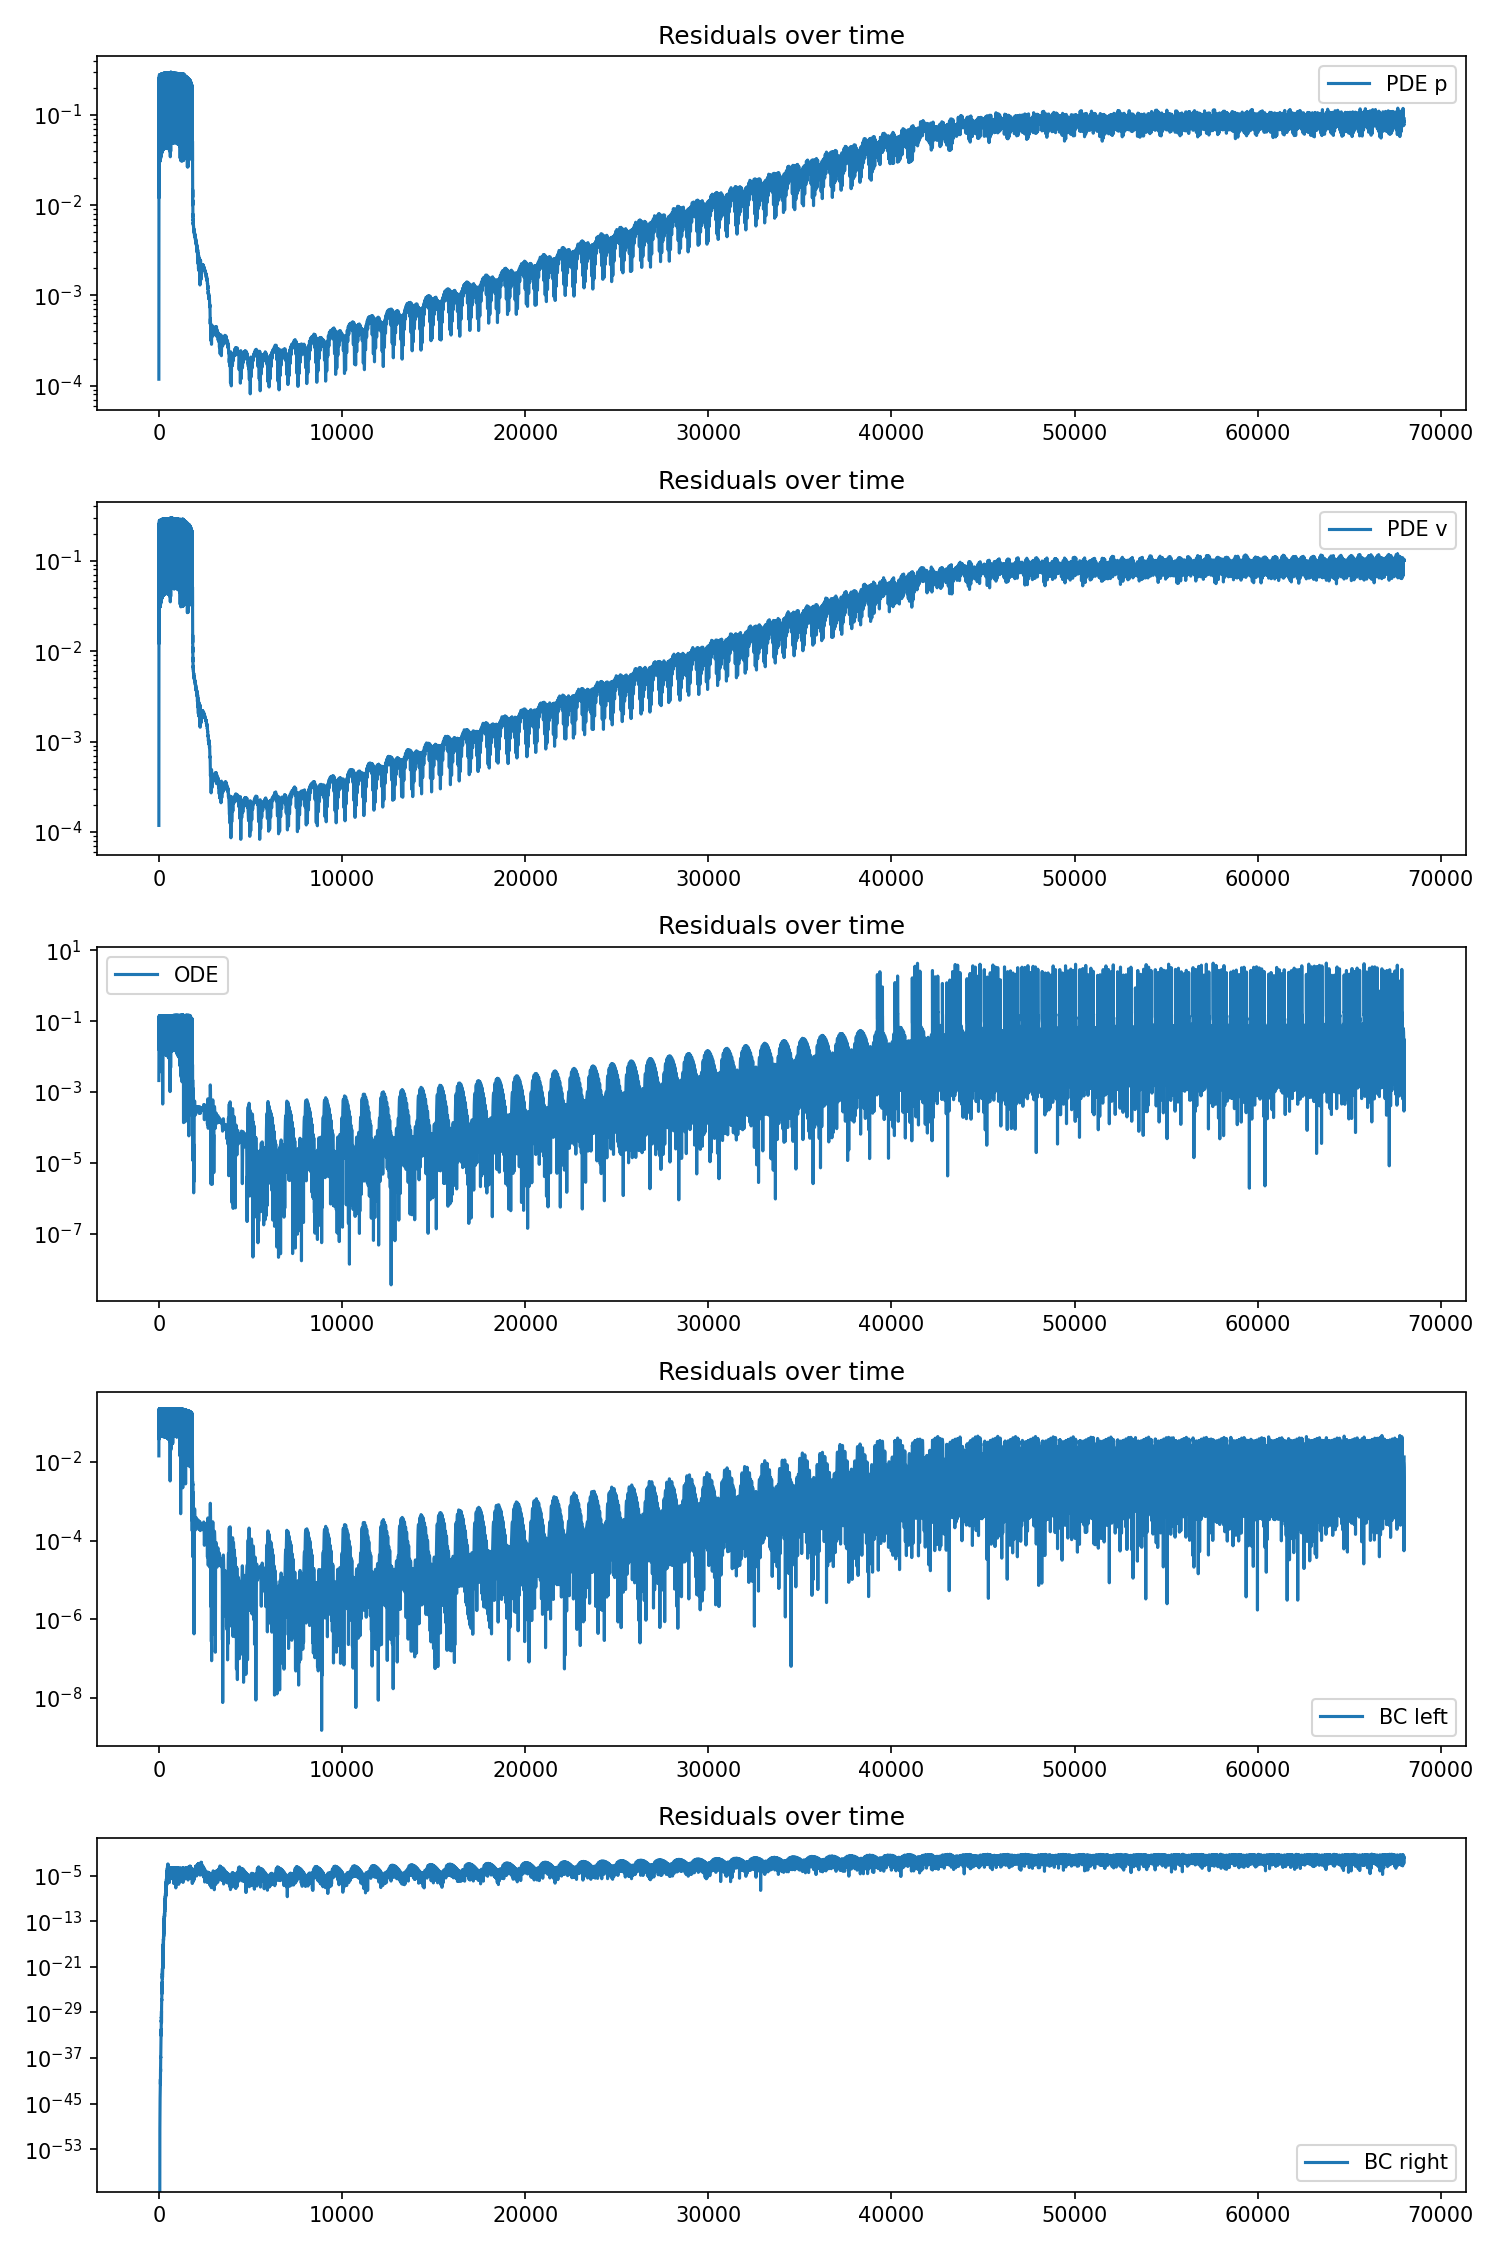
\includegraphics[width=0.7\textwidth]{residuals_rk2_const.png}
    \caption{Résidus de l'ODE et des BCs pour $\gamma(t)$ exponentiel dans le cas section constante.}
\end{figure}

\newpage
\subsubsection{Cas $S(x)$ variable avec pavillon exponentiel}

\begin{figure}[h]
    \centering
    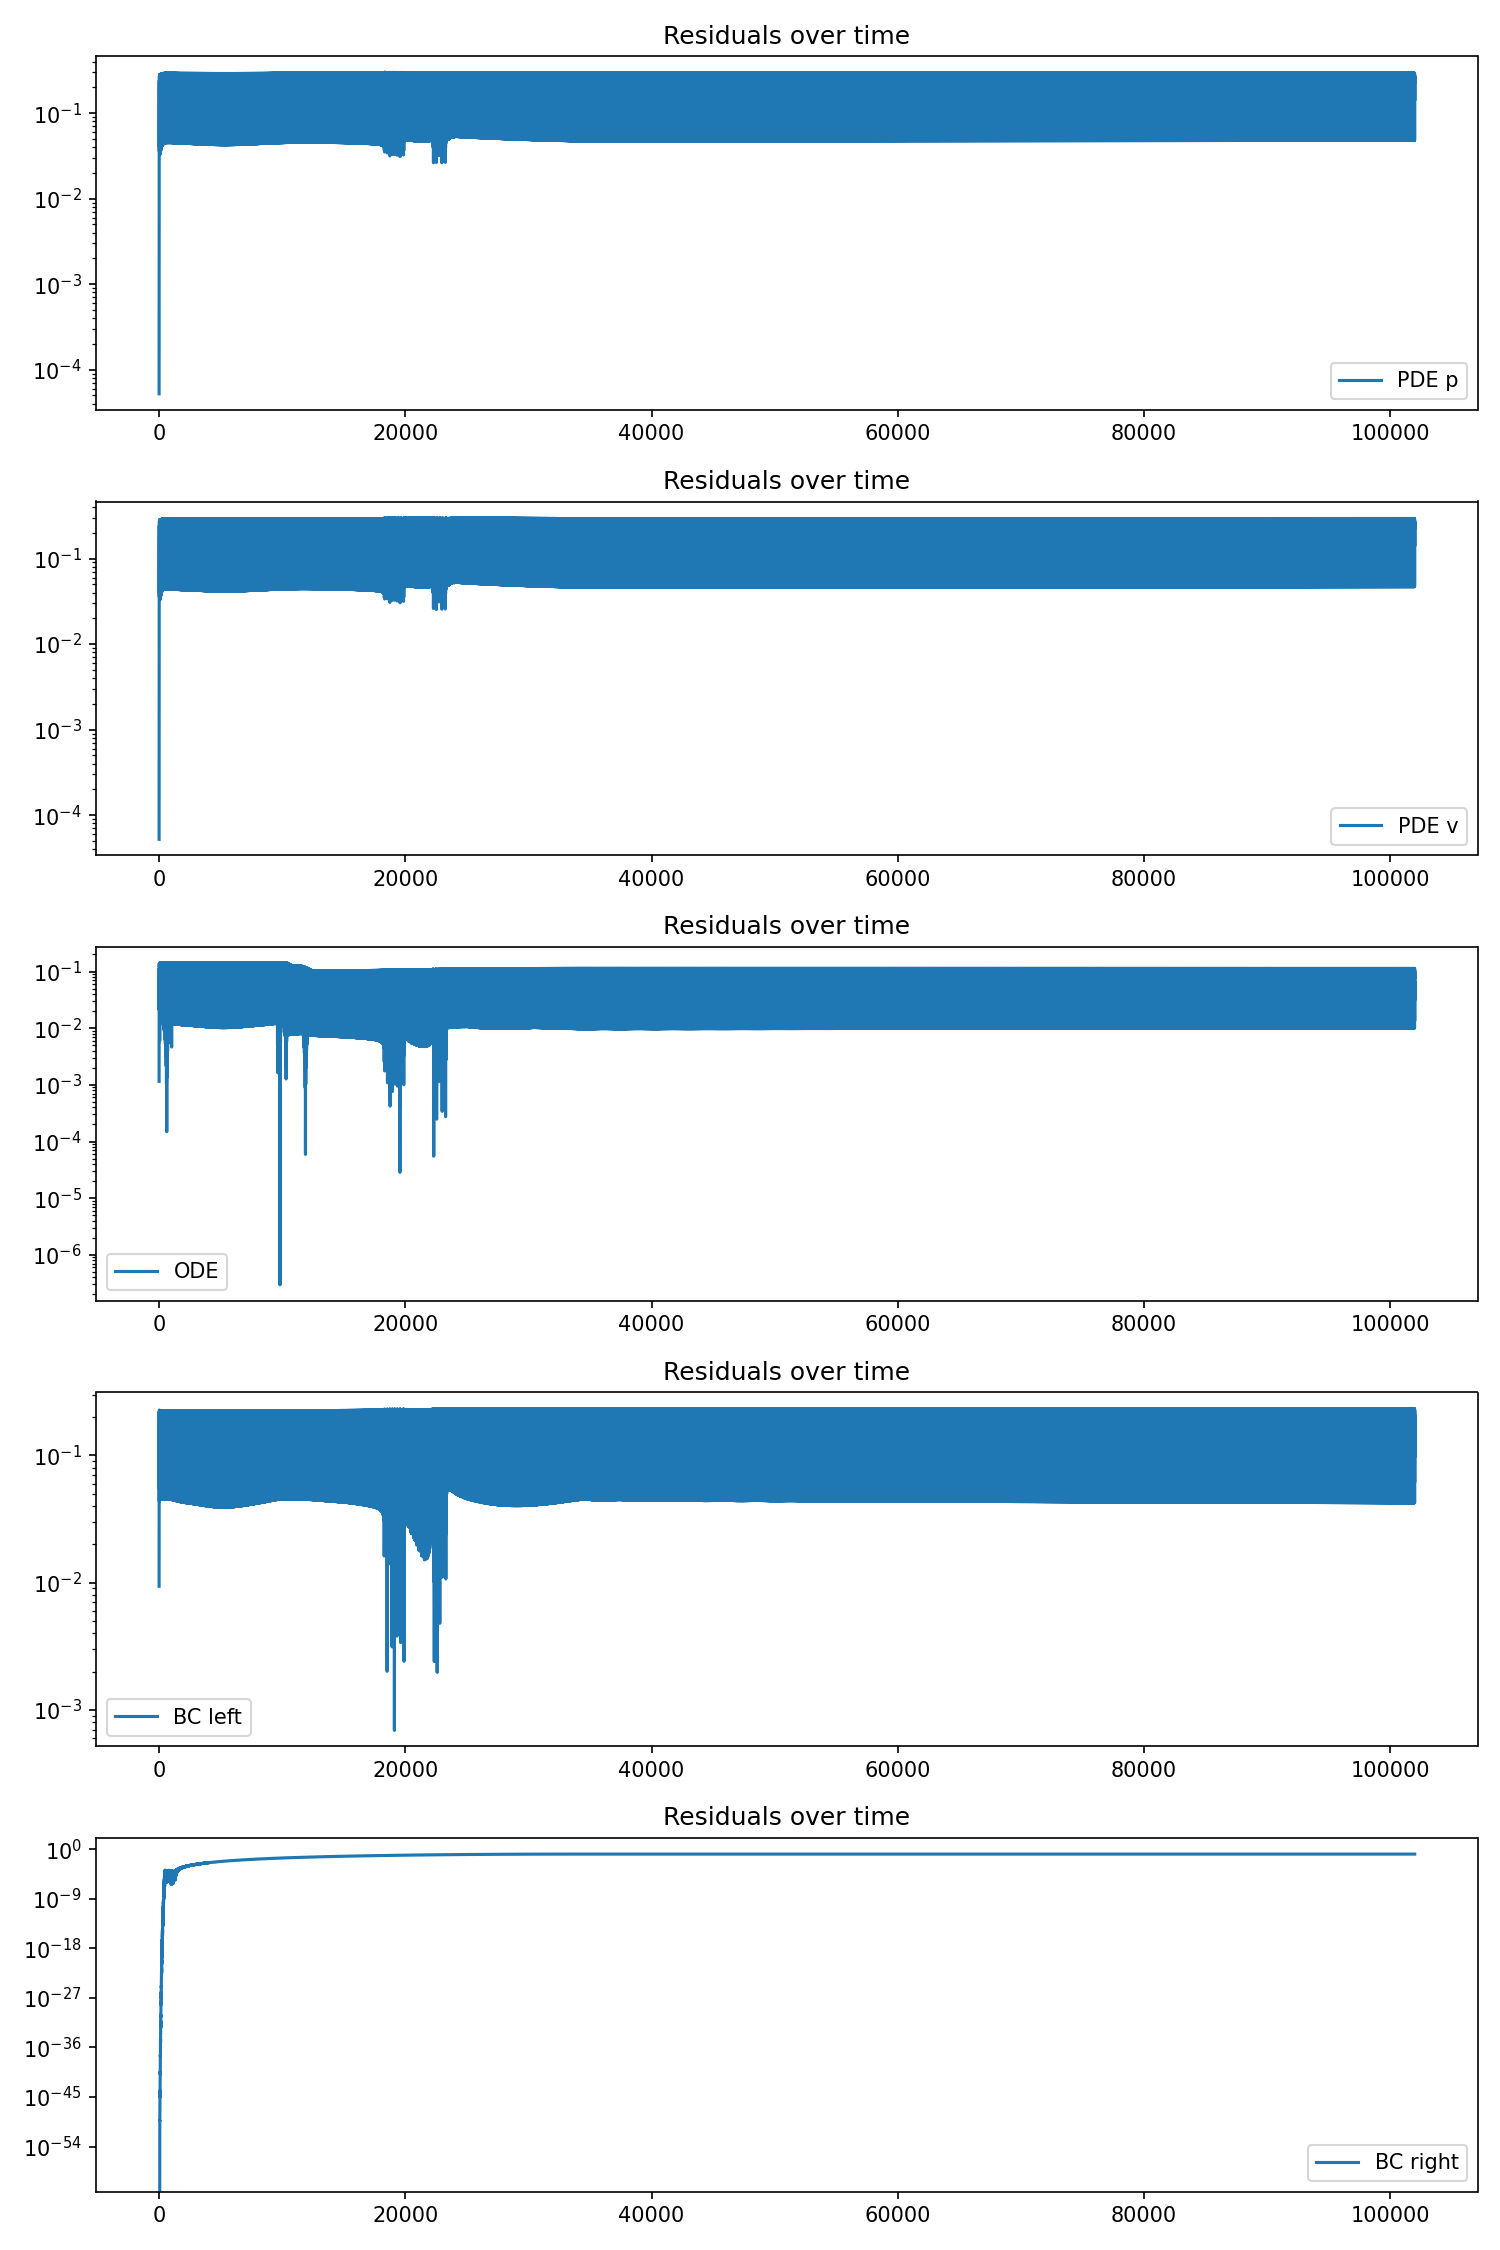
\includegraphics[width=0.7\textwidth]{residuals_rk2_exp.png}
    \caption{Résidus de l'ODE et des BCs pour $\gamma(t)$ exponentiel dans le cas section variable.}
\end{figure}

\newpage
\section{Sujet 4 : Résultats numériques comparées à OPENwind}

\newpage
\section{Sujet 5 : Calcul du gradient}


\newpage
\section{Questions}
Dans le papier CONTROL PARAMETERS FOR REED WIND INSTRUMENTS OR ORGAN PIPES WITH
REED INDUCED FLOW de Juliette Chabassier and Roman Auvray, on se rend compte que 
les paramètres implémenté dans mon modele proviennent de l'adimensionnalisation des
équations de base. Ce qui laisse sous entendre que pour la calibration, il faudra 
commencer par une étape de prétraitement sur la quantité d'intérêt à partir de 
laquelle on fera la calibration. 

\subsection{Paramètres physiques}

\begin{table}[h!]
    \centering
    \begin{tabular}{|c|c|c|}
        \hline
        \textbf{Paramètre} & \textbf{symbole} & \textbf{Valeur typique} \\
        \hline
        Densité de l'air & $\rho$ & $1.225 \, \text{kg/m}^3$ \\
        \hline
        Vitesse du son & $c$ & $343 \, \text{m/s}$ \\
        \hline
        Section de l'anche & $S_r$ & $1 \times 10^{-4} \, \text{m}^2$ \\
        \hline
        Masse de l'anche & $M_r$ & $3.376 \times 10^{-6} \, \text{kg}$ \\
        \hline
        Largeur de l'anche & $w$ & $0.002 \, \text{m}$ \\
        \hline
        Ouverture de l'anche & $y_0$ & $0.0004 \, \text{m}$ \\
        \hline
        Impédendce & $Z_T^\ast = \frac{\rho c}{S^\ast}$ & $2.65 \times 10^6 \, \text{kg/}(\text{m}^4\text{s})$ \\
        \hline
        Section du tube & $S^\ast$ & $1.54 \times 10^{-4} \, \text{m}^2$ \\
        \hline 
        pulsation propre de l'anche & $\omega_r$ & $2\pi \times 3700 \, \text{rad/s}$ \\
        \hline
        Pression de soufflage & $P_m$ & $2000 \, \text{Pa}$ \\
        \hline
        \end{tabular}
    \caption{Récapitulatif des paramètres physiques et leurs valeurs typiques.}
\end{table}

\subsection{Paramètres adimensionnalisés}

\begin{table}[h!]
    \centering
    \begin{tabular}{|c|c|c|}
        \hline
        \textbf{Paramètre adimensionnalisé} & \textbf{Formule} & \textbf{Échelle de valeurs} \\
        \hline
        $P^\ast$ (pression de référence) & $P^\ast = \frac{M_r}{S_r}y_0\omega_0^2$ & $4740$ Pa \\
        \hline
        $Q_r$ (facteur de qualité anche) & $Q_r = \frac{\omega_0}{g}$ & $7.71$ \\
        \hline
        $\kappa$ & $\kappa = \frac{Z_T^\ast S_r^2}{M_r \omega_0}$ & $0.71$ \\
        \hline
        $\zeta$ & $\zeta = Z_T^\ast w y_0 \sqrt{\frac{2}{\rho P^\ast}}$ & $0.4$ \\
        \hline
        $\gamma$ & $\gamma = \frac{P_m}{P^\ast}$ & $0.422$ \\
        \hline
        $\alpha$ & $\alpha = \frac{c}{R \delta_c}$ & $8 \times 10^4$ \\
        \hline
        $\beta$ & $\beta = \frac{\beta_c}{\delta_c^2}$ & $0.665$ \\
        \hline
    \end{tabular}
    \caption{Récapitulatif des paramètres adimensionnalisés et leurs échelles de valeurs typiques.}
\end{table}

Pour le calcul de $\alpha$ et $\beta$ j'ai utilisé des valeurs proposées dans la thèse d'Alexis 
à savoir $\delta_c = 0.6133$ et $\beta_c = 0.25$



\newpage
\section{Sujet 6 : Paramètres de simulation}

\subsection{Configuration générale}

\begin{table}[h!]
    \centering
    \begin{tabular}{|c|c|c|}
        \hline
        \textbf{Paramètre} & \textbf{Symbole} & \textbf{Valeur} \\
        \hline
        Vitesse du son & $c$ & $340.0 \, \text{m/s}$ \\
        \hline
        Section du tube & $S^*$ & $0.035 \, \text{m}^2$ \\
        \hline
        Condition initiale (phi) & $\phi_0$ & $0.0$ \\
        \hline
        Temps maximum de simulation & $T_{\max}$ & $1.0 \, \text{s}$ \\
        \hline
        Nombre de Courant & $\text{CFL}$ & $0.2$ \\
        \hline
    \end{tabular}
    \caption{Paramètres du solveur numérique.}
\end{table}

\subsection{Géométrie de l'instrument}

\begin{table}[h!]
    \centering
    \begin{tabular}{|c|c|c|}
        \hline
        \textbf{Paramètre} & \textbf{Symbole} & \textbf{Valeur} \\
        \hline
        Longueur du tube & $L_{\text{tube}}$ & $0.4 \, \text{m}$ \\
        \hline
        Rayon du tube & $R_{\text{tube}}$ & $0.007 \, \text{m}$ \\
        \hline
        Longueur du pavillon & $L_{\text{bell}}$ & $0.1 \, \text{m}$ \\
        \hline
        Coefficient exponentiel du pavillon & $k_{\text{bell}}$ & $20.0$ \\
        \hline
    \end{tabular}
    \caption{Paramètres géométriques de l'instrument.}
\end{table}

\subsection{Conditions aux limites gauche (anche)}

\begin{table}[h!]
    \centering
    \begin{tabular}{|c|c|c|}
        \hline
        \textbf{Paramètre} & \textbf{Symbole} & \textbf{Valeur} \\
        \hline
        Pression finale de soufflage & $\gamma_{\text{final}}$ & $0.422$ \\
        \hline
        Temps d'attaque & $t_{\text{attack}}$ & $0.02 \, \text{s}$ \\
        \hline
        Coefficient de couplage anche-tube & $\epsilon$ & $-1.0$ \\
        \hline
        Paramètre anche & $\kappa$ & $0.71$ \\
        \hline
        Fréquence propre de l'anche & $f_r$ & $170.0 \, \text{Hz}$ \\
        \hline
        Facteur de qualité de l'anche & $Q_r$ & $125.0$ \\
        \hline
        Paramètre d'ouverture & $\zeta$ & $0.4$ \\
        \hline
    \end{tabular}
    \caption{Paramètres des conditions aux limites gauche.}
\end{table}

\newpage
\subsection{Conditions aux limites droite (pavillon)}

\begin{table}[h!]
    \centering
    \begin{tabular}{|c|c|c|}
        \hline
        \textbf{Paramètre} & \textbf{Symbole} & \textbf{Valeur} \\
        \hline
        Coefficient de radiation & $\beta$ & $30.0$ \\
        \hline
        Impédance caractéristique & $Z_t$ & $1.0$ \\
        \hline
        Facteur d'amortissement & $\alpha$ & $0.0333$ \\
        \hline
    \end{tabular}
    \caption{Paramètres des conditions aux limites droite.}
\end{table}

\subsection{Conditions initiales de l'anche}

\begin{table}[h!]
    \centering
    \begin{tabular}{|c|c|c|}
        \hline
        \textbf{Paramètre} & \textbf{Symbole} & \textbf{Valeur} \\
        \hline
        Ouverture initiale de l'anche & $y_0$ & $1.0$ \\
        \hline
        Vitesse initiale de l'anche & $\dot{y}_0$ & $0.0$ \\
        \hline
    \end{tabular}
    \caption{Conditions initiales de l'anche.}
\end{table}
\end{document}